\chapter{Convergencia de MCMC} \label{Anexo_Convergencia}

La convergencia de los promedios ergódicos que implica \eqref{eq:Teo_Erg_Conv_Prom} es la clave de un análisis de MCMC, pues nos permite aproximar los resúmenes inferenciales que necesitamos, tanto como nuestros recursos computacionales lo permitan. Sin embargo, como menciono en el texto principal, en un análisis bayesiano la única receta indica tener una muestra aleatoria de la distribución posterior. Si observamos con cuidado \eqref{eq:Teo_Erg_Conv_D}, vemos que la última simulación de la cadena es la que podemos considerar como proveniente de la distribución objetivo límite. Si quisiéramos una muestra de tamaño $N$, podríamos inicialmente pensar que necesitaríamos correr $N$ cadenas independientes.\\ 

Afortunadamente, en las cadenas de MCMC en general, la distribución límite es también lo que se conoce como \textit{distribución estacionaria} de la cadena de Markov. Esto quiere decir que el kernel de transición de la cadena mantiene estable la distribución de las simulaciones, una vez que se alcanza la distribución estacionaria \parencite{Neal93}. Esta característica estacionaria de la distribución límite implica que si reiniciamos la cadena una vez que se llega a la convergencia, podemos después de algún número de transiciones adicionales contar con otra observación prácticamente independiente proveniente de la misma distribución objetivo.\\ 

Por consiguiente, aunque los algoritmos de MCMC producen cadenas correlacionadas, es posible calcular un \textit{tamaño efectivo de muestra} que aproxima el tamaño de una muestra aleatoria auténticamente independiente proveniente de la distribución objetivo cuyas estimaciones equivaldrían a las que hacemos con la muestra simulada. Los detalles de cómo se calcula dicha estadística puede consultarse en \textcite{Gelman13}.\\ 

Por lo anterior, usualmente solo se conservan las simulaciones cada $m$ transiciones de manera que la correlación entre ellas sea lo más cercana a cero posible. Buscaríamos descartar aquellas simulaciones que, debido a la correlación, no están aportando realmente mayor información sobre la distribución objetivo. Con este \textit{adelgazamiento} de la cadena se busca ahorrar espacio de memoria en la computadora y conservar solo las simulaciones que aportan \textit{nueva} información y aumentan el tamaño efectivo de muestra.\\ 

En este sentido, la forma usual de aplicar la inferencia bayesiana mediante MCMC se resume de la manera siguiente: 

\begin{enumerate}
\item Elegir un número $c$ de cadenas para simular.
\item Iniciar cada cadena en un punto distinto y disperso del espacio parametral. 
\item Correr de manera independiente las $c$ cadenas hasta que ``alcancen la convergencia''. 
\item Una vez que se considera que las cadenas convergieron, se desechan las transiciones iniciales que constituyen el \textit{periodo de calentamiento}. 
\item Se \textit{adelgaza} cada cadena conservando las simulaciones solo cada $m$ transiciones de manera que la correlación sea baja. 
\item Se continúan realizando simulaciones después del calentamiento y el adelgazamiento hasta obtener una muestra ``lo suficientemente grande''.  
\end{enumerate}

El número de cadenas se puede elegir en función del número de procesos paralelos que la computadora puede realizar para aprovechar la eficiencia que implica el cómputo paralelo. Usualmente se corren 3, 4 o 5 cadenas. Por su parte, seleccionar el espaciamiento $m$ de las cadenas normalmente implica realizar gráficos de autocorrelación para algunas pruebas preliminares cuyo objetivo es también determinar la convergencia del algoritmo. En realidad, el punto más delicado es precisamente este último, declarar la convergencia.\\ 

Desafortunadamente, los teoremas ergódicos son asintóticos, por lo que solo se garantiza la convergencia en el infinito. Aunque hay cotas para los errores, normalmente no son muy útiles, salvo algunos casos \parencite{SmithRoberts93}. Por ello, en la práctica se han desarrollado diferentes técnicas de diagnóstico de convergencia. Sin embargo, ninguna puede garantizarnos totalmente que la cadena ya haya convergido. Entonces, es recomendable considerar diferentes técnicas para disminuir la probabilidad de pasar por alto algún problema de convergencia. Una vez que estamos satisfechos con las pruebas de convergencia, podemos utilizar todas las simulaciones como una sola muestra que caracteriza la distribución posterior y realizar las estimaciones de Monte Carlo necesarias.\\

La primera técnica ya la he utilizado en los ejemplos de RWM y Gibbs: graficar los promedios ergódicos para diferentes variables o resúmenes inferenciales para observar en qué punto se estabilizan. La segunda es precisamente iniciar en puntos dispersos del espacio parametral para evitar que las cadenas exploren solo una parte del espacio y, por ejemplo, queden atrapadas en una sola moda cuando la distribución posterior pueda ser multimodal. Al mismo tiempo, tener diferentes cadenas nos permite comparar las estimaciones dentro de cada cadena así como a través de las cadenas. Un ejemplo de promedios ergódicos para 4 cadenas de \textit{Gibbs Sampler} (GS) iniciadas en puntos dispersos del espacio parametral puede verse en la \textbf{Figura \ref{fig:Conv_Prom_Erg}}.\\ 

\begin{figure}[h]
	\centering
	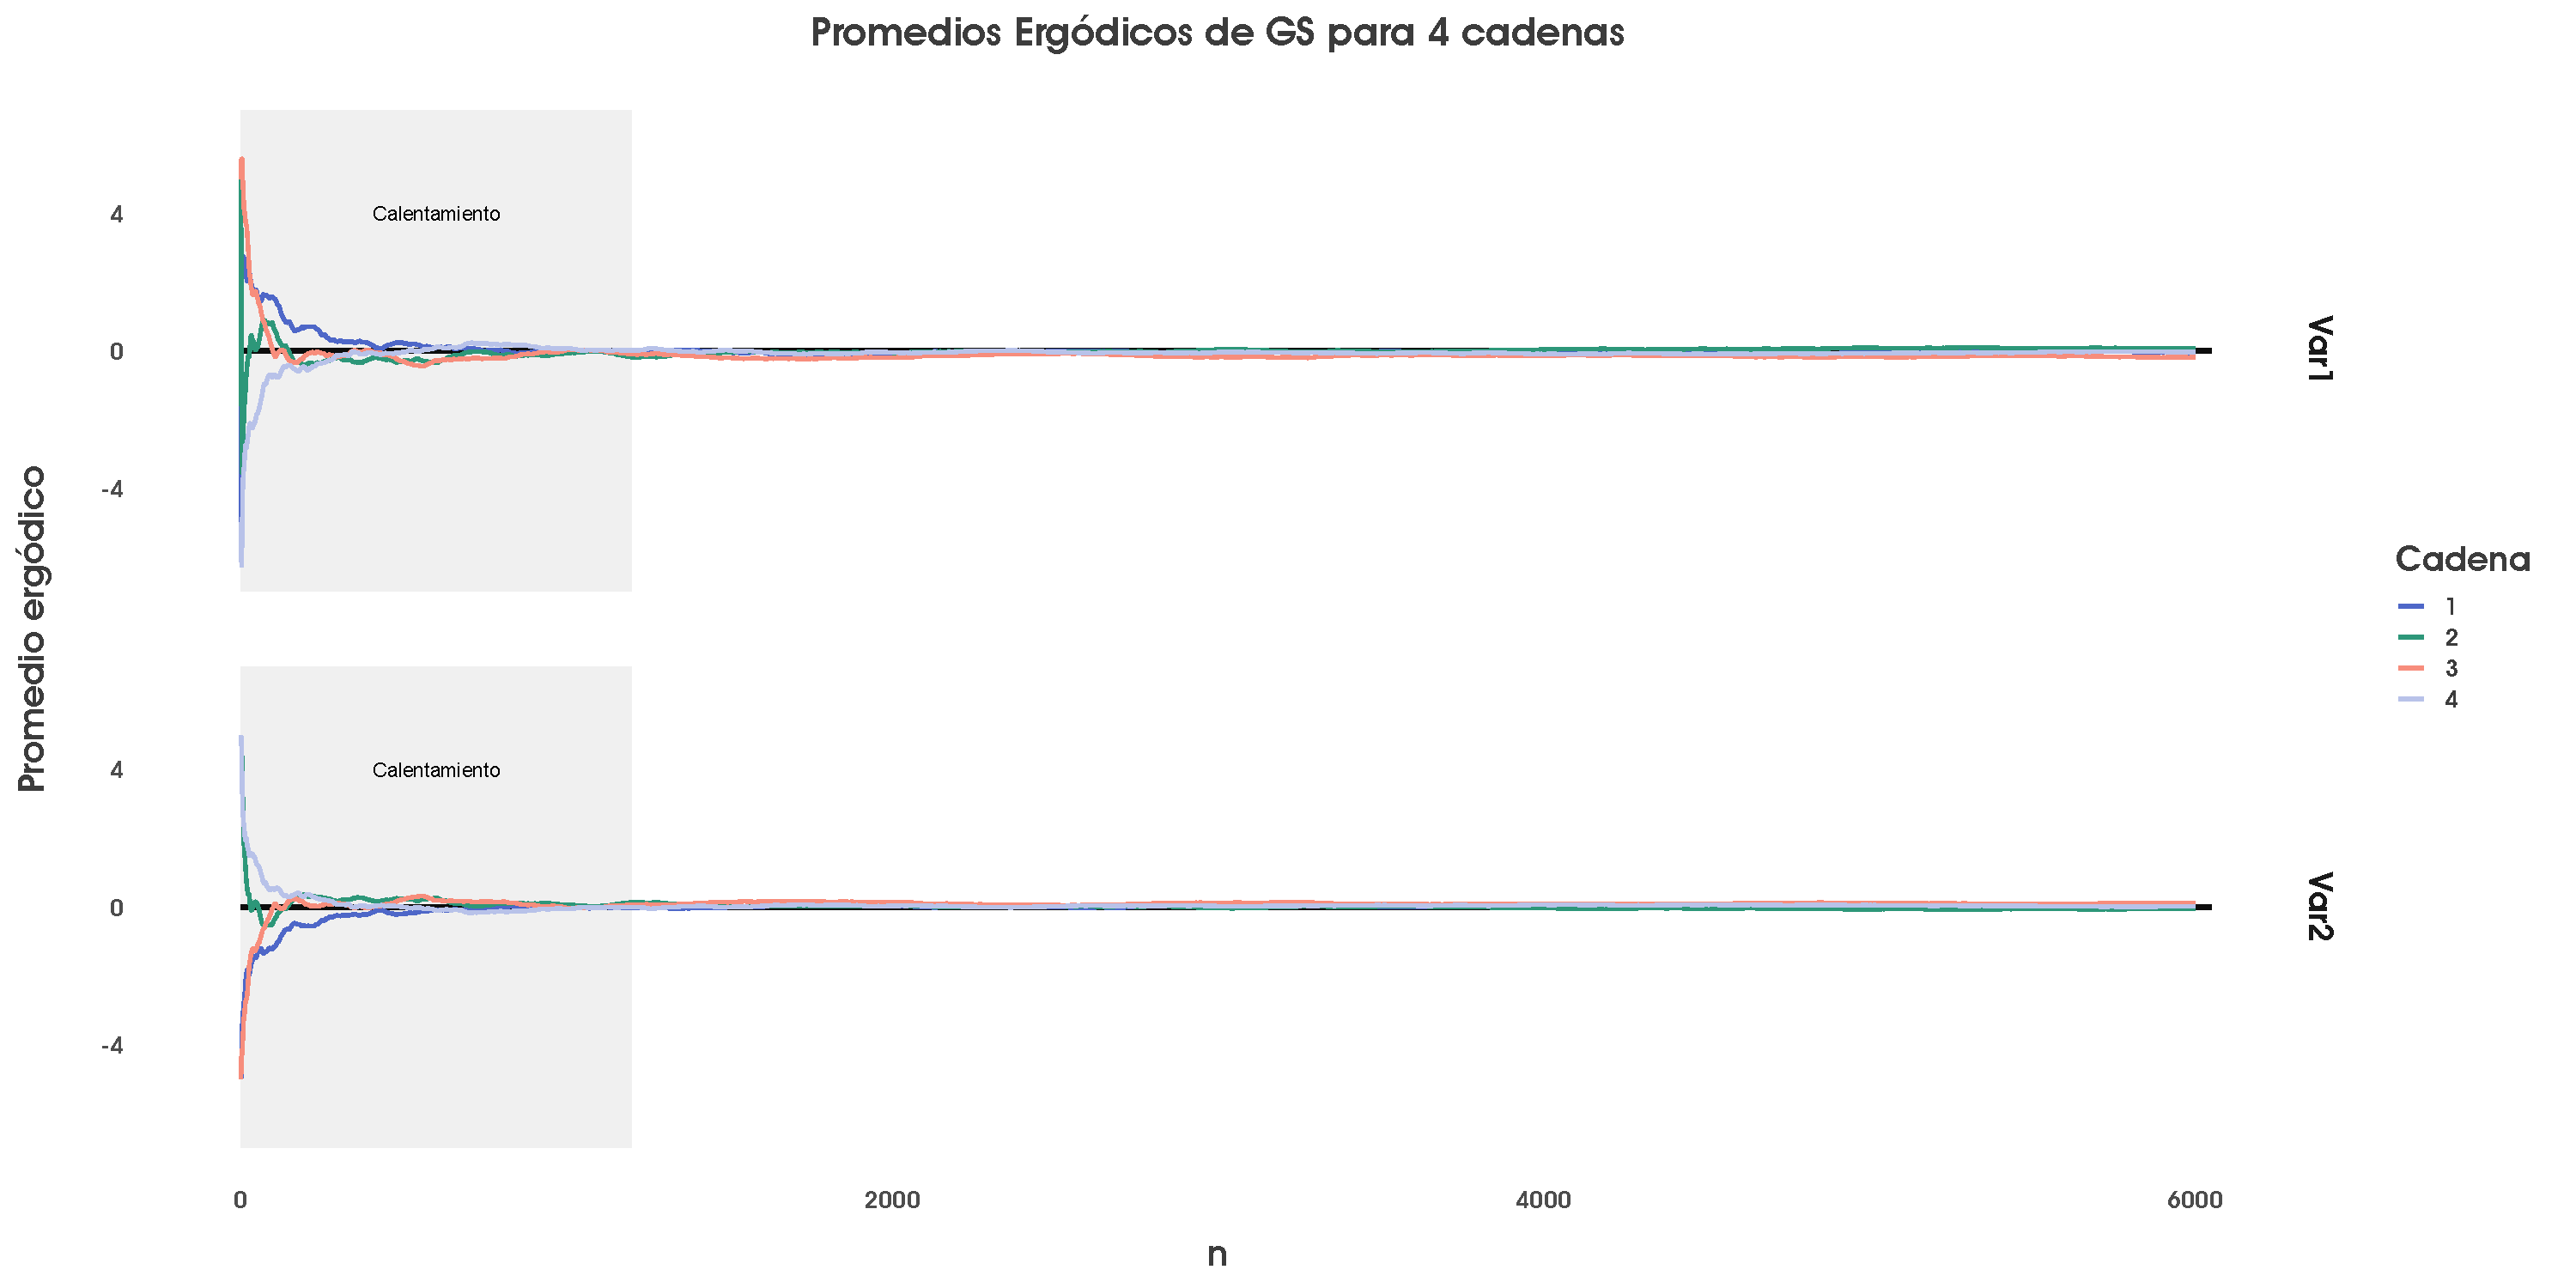
\includegraphics[width=0.9\textwidth]{Figs/Bayes/Ejemplos_Convergencia_Prom_Erg}
	\caption{Ilustración de la convergencia de dos promedios ergódicos para 4 cadenas de \textit{Gibbs Sampling} iniciadas en puntos dispersos del espacio parametral. Vemos cómo las estimaciones de distintas cadenas se estabilizan y mezclan. Esto ayuda a detectar la fase de calentamiento. Fuente: elaboración propia.}
	\label{fig:Conv_Prom_Erg}	
\end{figure}

En el fondo, hay dos características que se buscan para declarar la convergencia \parencite{Gelman13}. Queremos que las cadenas lleguen a la estacionariedad, pues la distribución límite es también estacionaria. Las estimaciones deben estabilizarse. También, y dicho de manera coloquial, buscamos que las cadenas \textit{mezclen} bien. Es decir, que las estimaciones para cada cadena sean parecidas a las estimaciones de todas las cadenas en su conjunto. Por ello un buen algoritmo de MCMC buscará recorrer y explorar todas las regiones críticas de la distribución objetivo \parencites{Neal93,Betancourt18}.\\ 

Uno de los diagnósticos visuales más utilizados son los llamados gráficos de oruga o \textit{trace plots}. En ellos se grafica la secuencia de iteraciones, es decir en el eje $x$ se encuentra el número de iteración y en el eje $y$ el valor o estado de la cadena en dicha iteración. Si las cadenas son estacionarias entonces el gráfico saltará de un punto a otro dentro de un rango de valores que determinan la región crítica. Si las cadenas mezclan bien, entonces las diferentes secuencias estarán oscilando en la misma región crítica, intercalándose. El \textit{trace plot} del ejemplo de esta sección puede verse en la \textbf{Figura \ref{fig:Conv_Trace_Inicial}}. También podemos ver en la \textbf{Figura \ref{fig:Conv_Trace_Final}}, el gráfico correspondiente a las iteraciones válidas para cada cadena, es decir, después del descarte del periodo de calentamiento y el espaciamiento para evitar la correlación.\\

\begin{figure}[h]
	\centering
	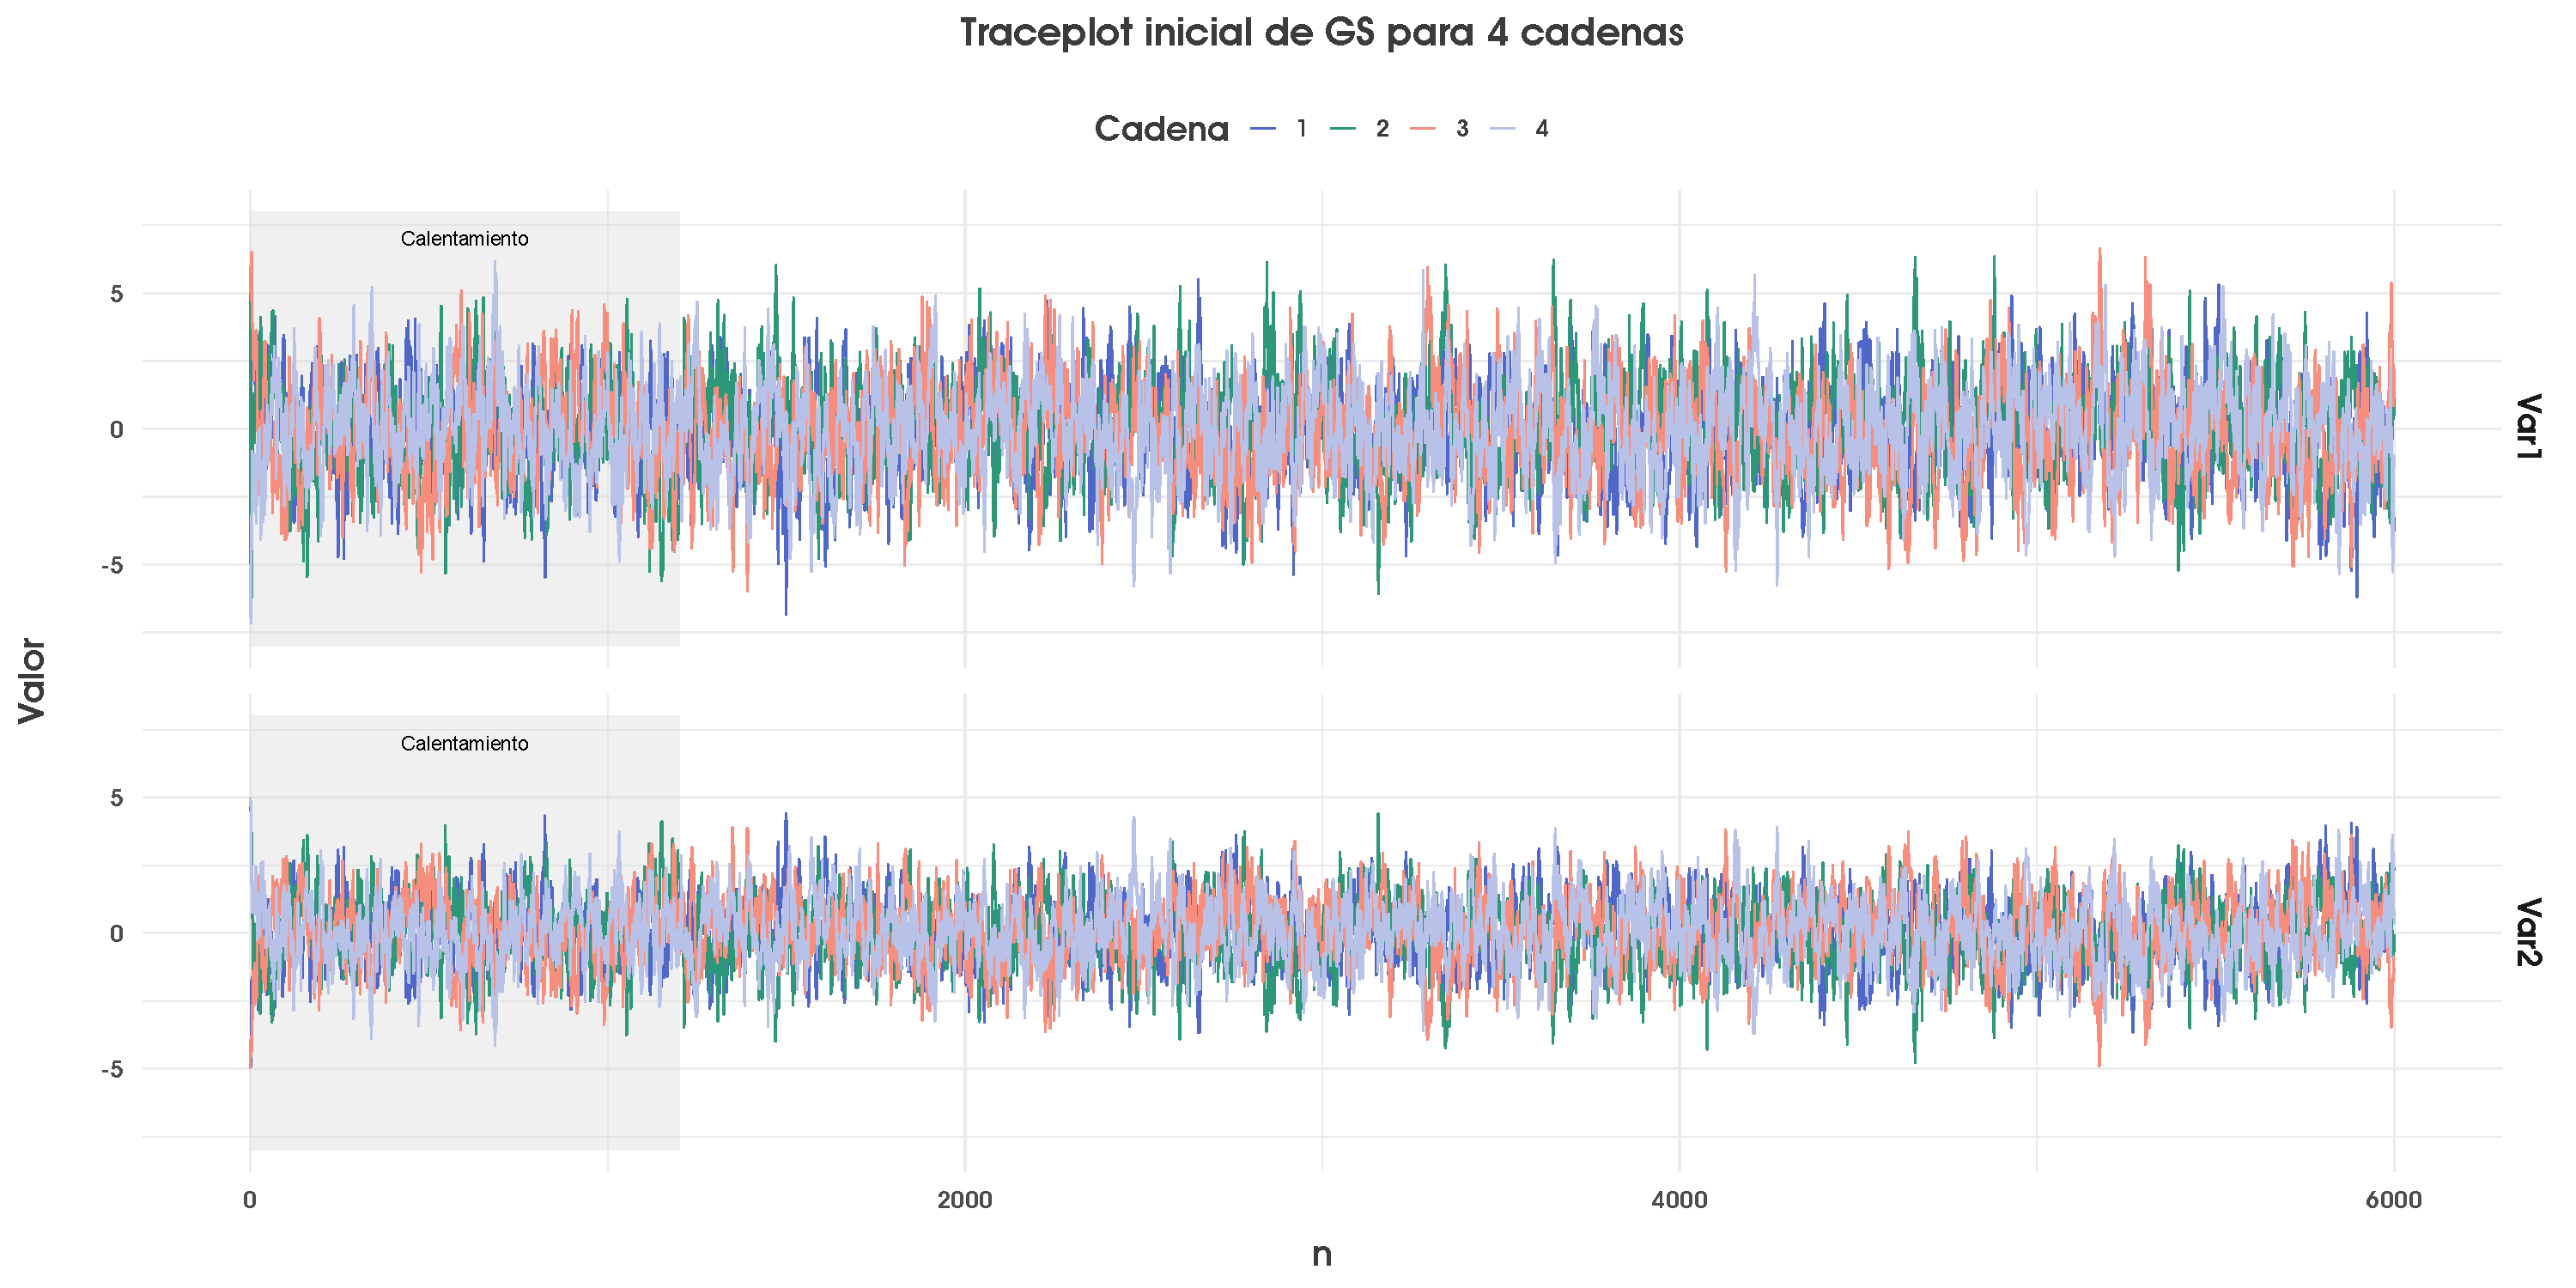
\includegraphics[width=0.9\textwidth]{Figs/Bayes/Ejemplos_Convergencia_Traceplot_Inicial}
	\caption{Ilustración de un \textit{trace plot} para las 4 cadenas de \textit{Gibbs Sampling}. Vemos el comportamiento de oruga, al rededor de una banda de valores. Fuente: elaboración propia.}
	\label{fig:Conv_Trace_Inicial}	
\end{figure}

\begin{figure}[h]
	\centering
	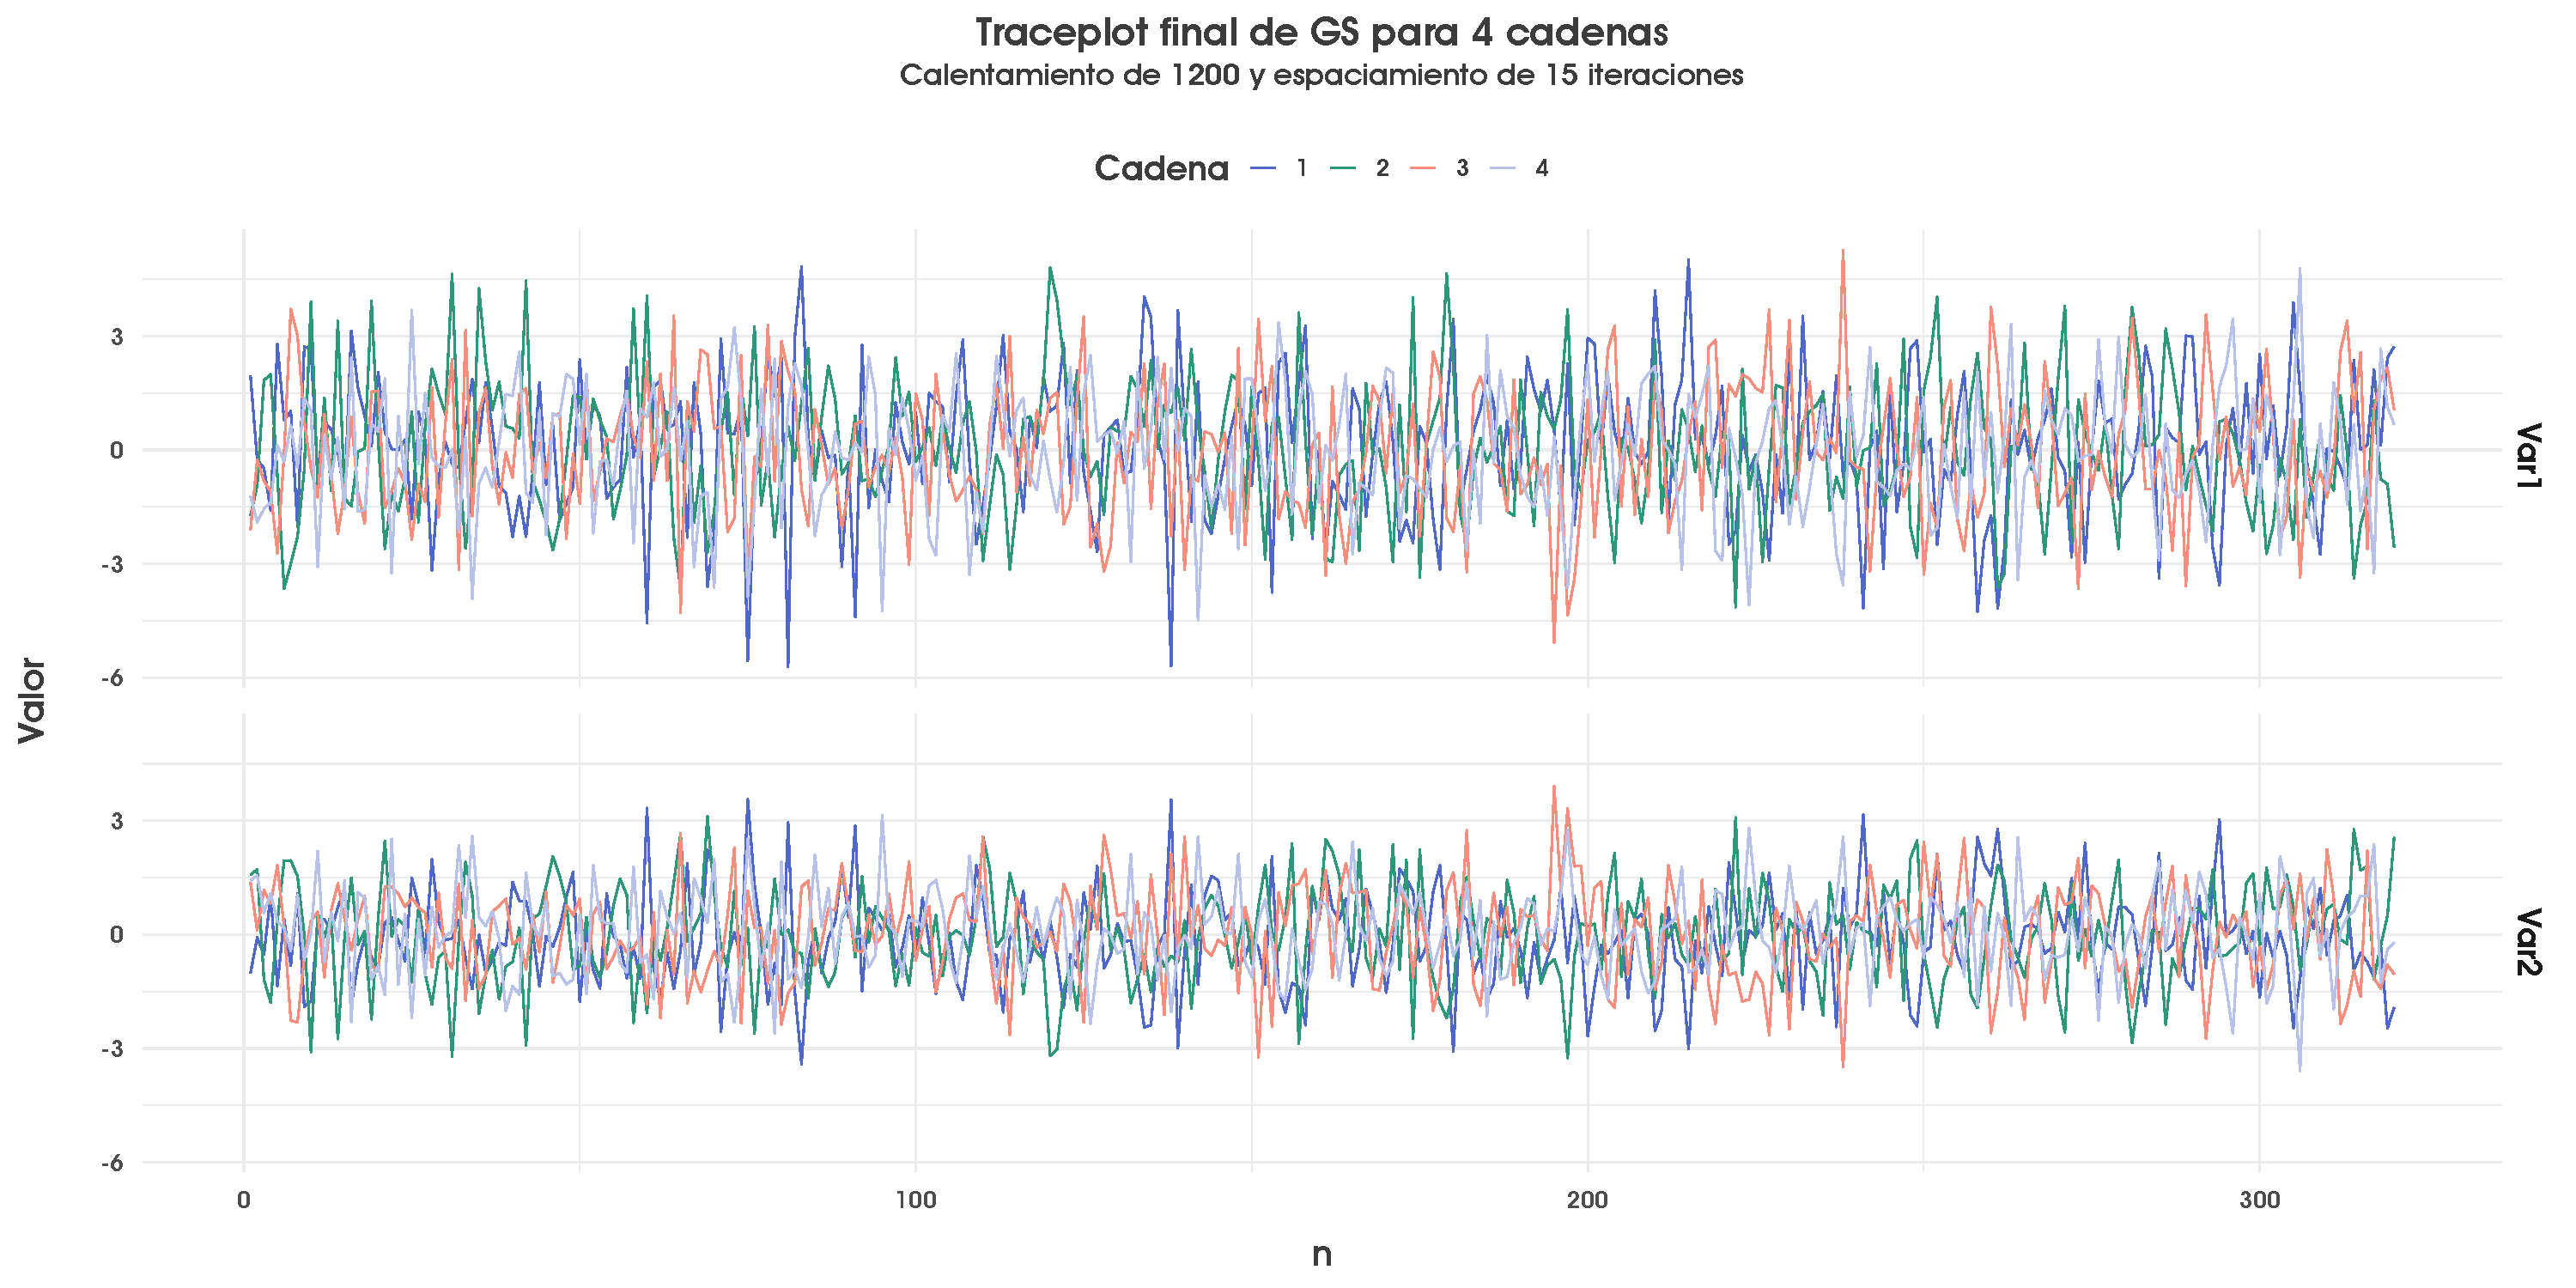
\includegraphics[width=0.9\textwidth]{Figs/Bayes/Ejemplos_Convergencia_Traceplot_Final}
	\caption{Ilustración de un \textit{trace plot} para las 4 cadenas de \textit{Gibbs Sampling} considerando solo las iteraciones válidas. Fuente: elaboración propia.}
	\label{fig:Conv_Trace_Final}	
\end{figure}

En este caso, el ejemplo es lo suficientemente sencillo para permitirnos un adelgazamiento de 8, aunque este suele ser más chico. La reducción en la autocorrelación que esto tiene se puede apreciar en la \textbf{Figura \ref{fig:Conv_Autocorr}}. En los gráficos de la cadena completa, del lado izquierdo, vemos que la autocorrelación es superior a 0.75 para un \textit{lag} de 1 e incluso sigue siendo mayor a 0.5 para algunas cadenas y \textit{lags} de 4. Por el contrario, del lado derecho, observamos que tras adelgazar la cadena las autocorrelaciones ya son siempre menores a 0.25 desde el primer \textit{lag}.\\ 

\begin{figure}[h]
    \centering
    \begin{subfigure}{0.45\textwidth}
        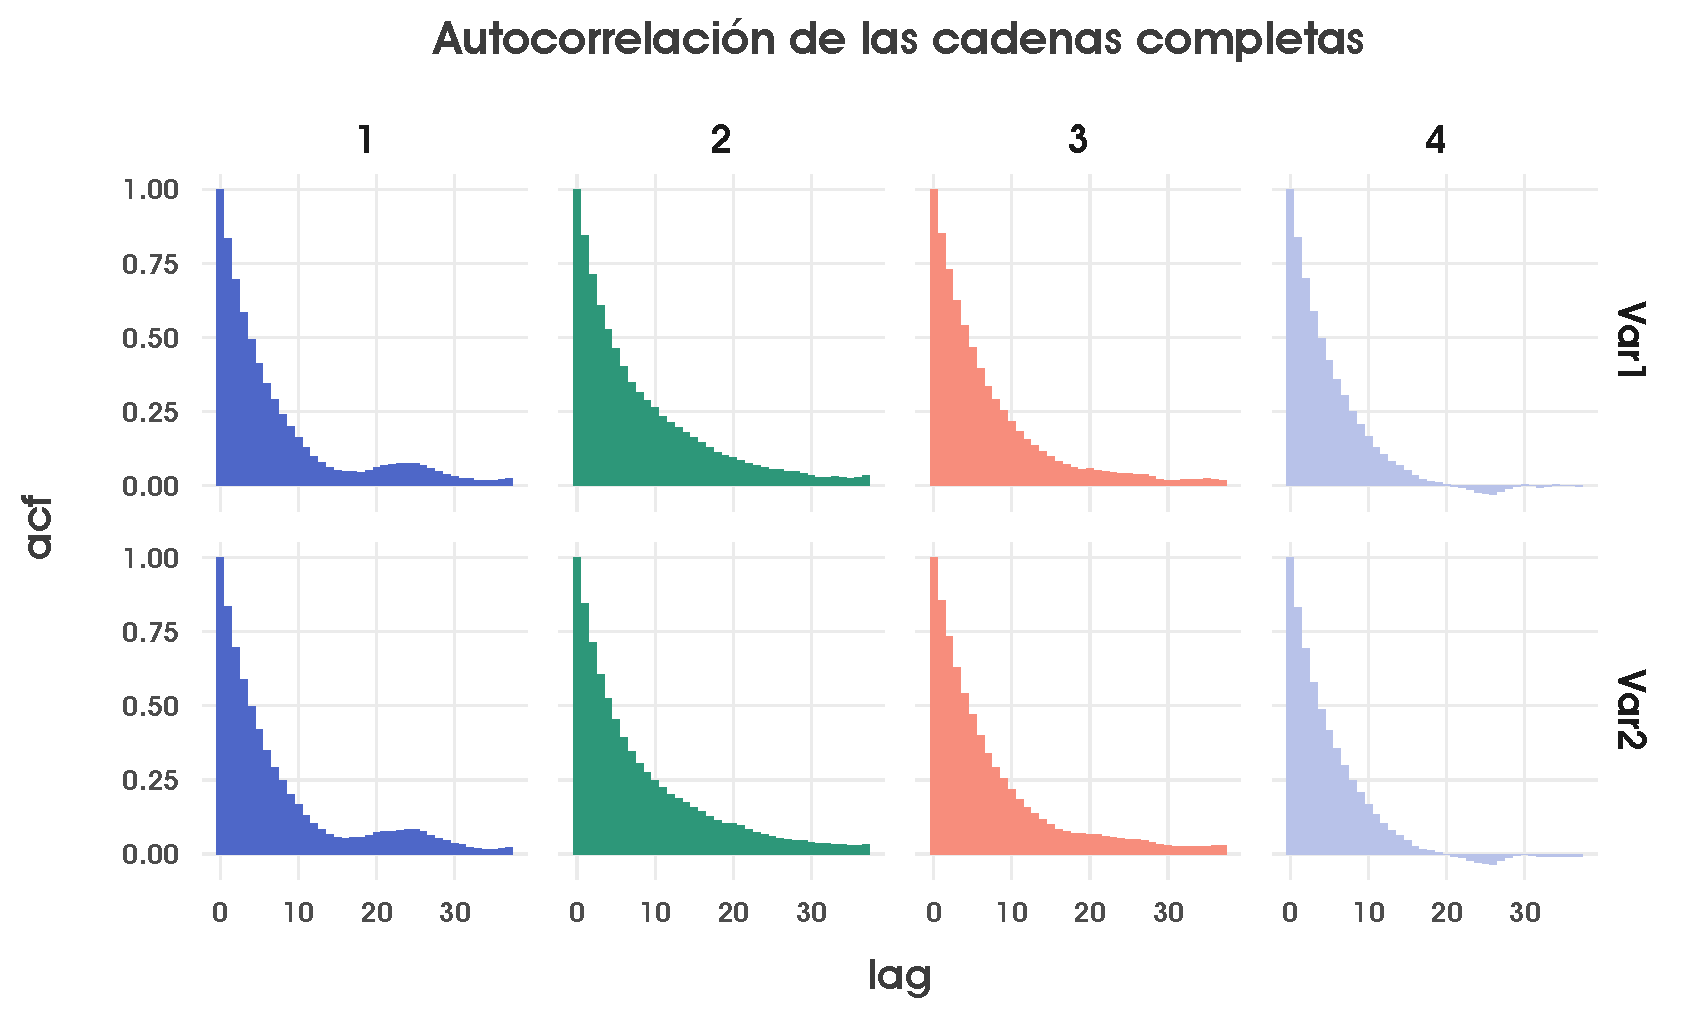
\includegraphics[width=\textwidth]{Figs/Bayes/Ejemplos_Convergencia_Autocorr_Completas}
    \end{subfigure}
    ~ 
    \begin{subfigure}{0.45\textwidth}
        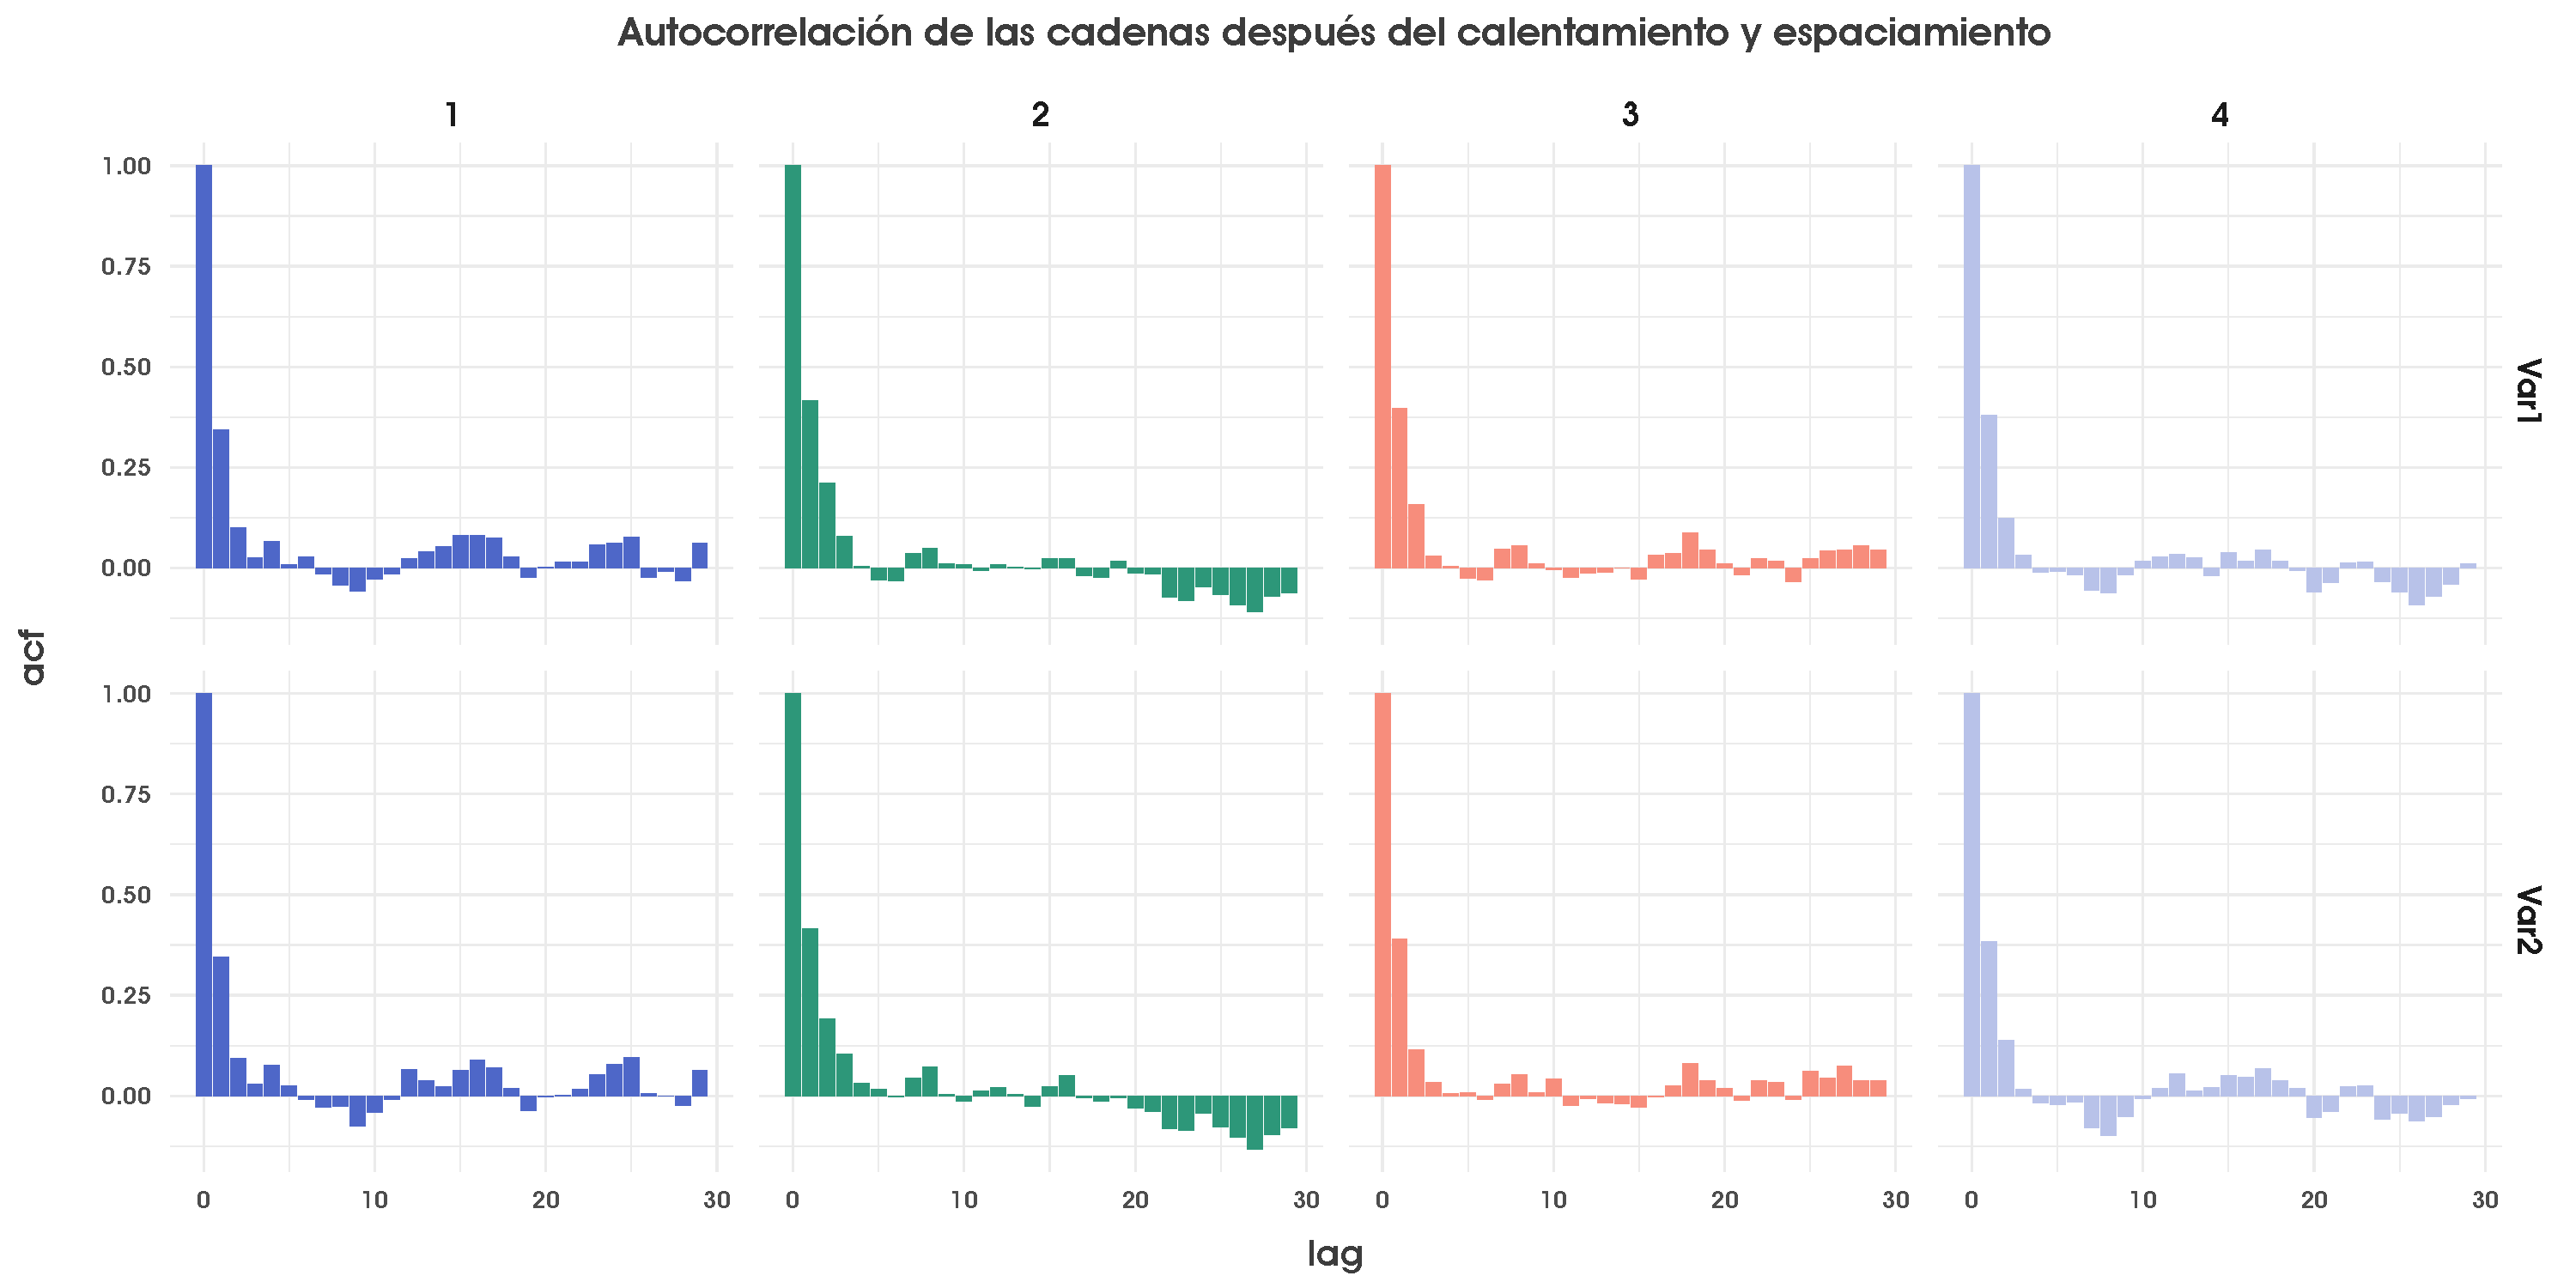
\includegraphics[width=\textwidth]{Figs/Bayes/Ejemplos_Convergencia_Autocorr_Final}
    \end{subfigure}
    \caption{Gráficos de autocorrelación para las 4 cadenas de \textit{Gibbs Sampling} antes y después de realizar un adelgazamiento de 8. Fuente: elaboración propia.}\label{fig:Conv_Autocorr}
\end{figure}

Otro diagnóstico gráfico es el de comparar histogramas o densidades estimadas para varios parámetros y resúmenes inferenciales y verificar que estos son estables--- comparándolos para la primera mitad de la muestra y para la segunda, por ejemplo--- y mezclan bien--- los gráficos para las diferentes cadenas se parecen al gráfico de todas juntas---. Para el ejemplo, vemos la comparación de los histogramas de cada cadena con el histograma de todas las cadenas en su conjunto en la \textbf{Figura \ref{fig:Conv_Hist}}. Si bien no son exactamente iguales, pues son simulaciones independientes, sí son muy parecidos entre sí lo que indica que las cadenas mezclaron bien.\\

\begin{figure}[h]
	\centering
	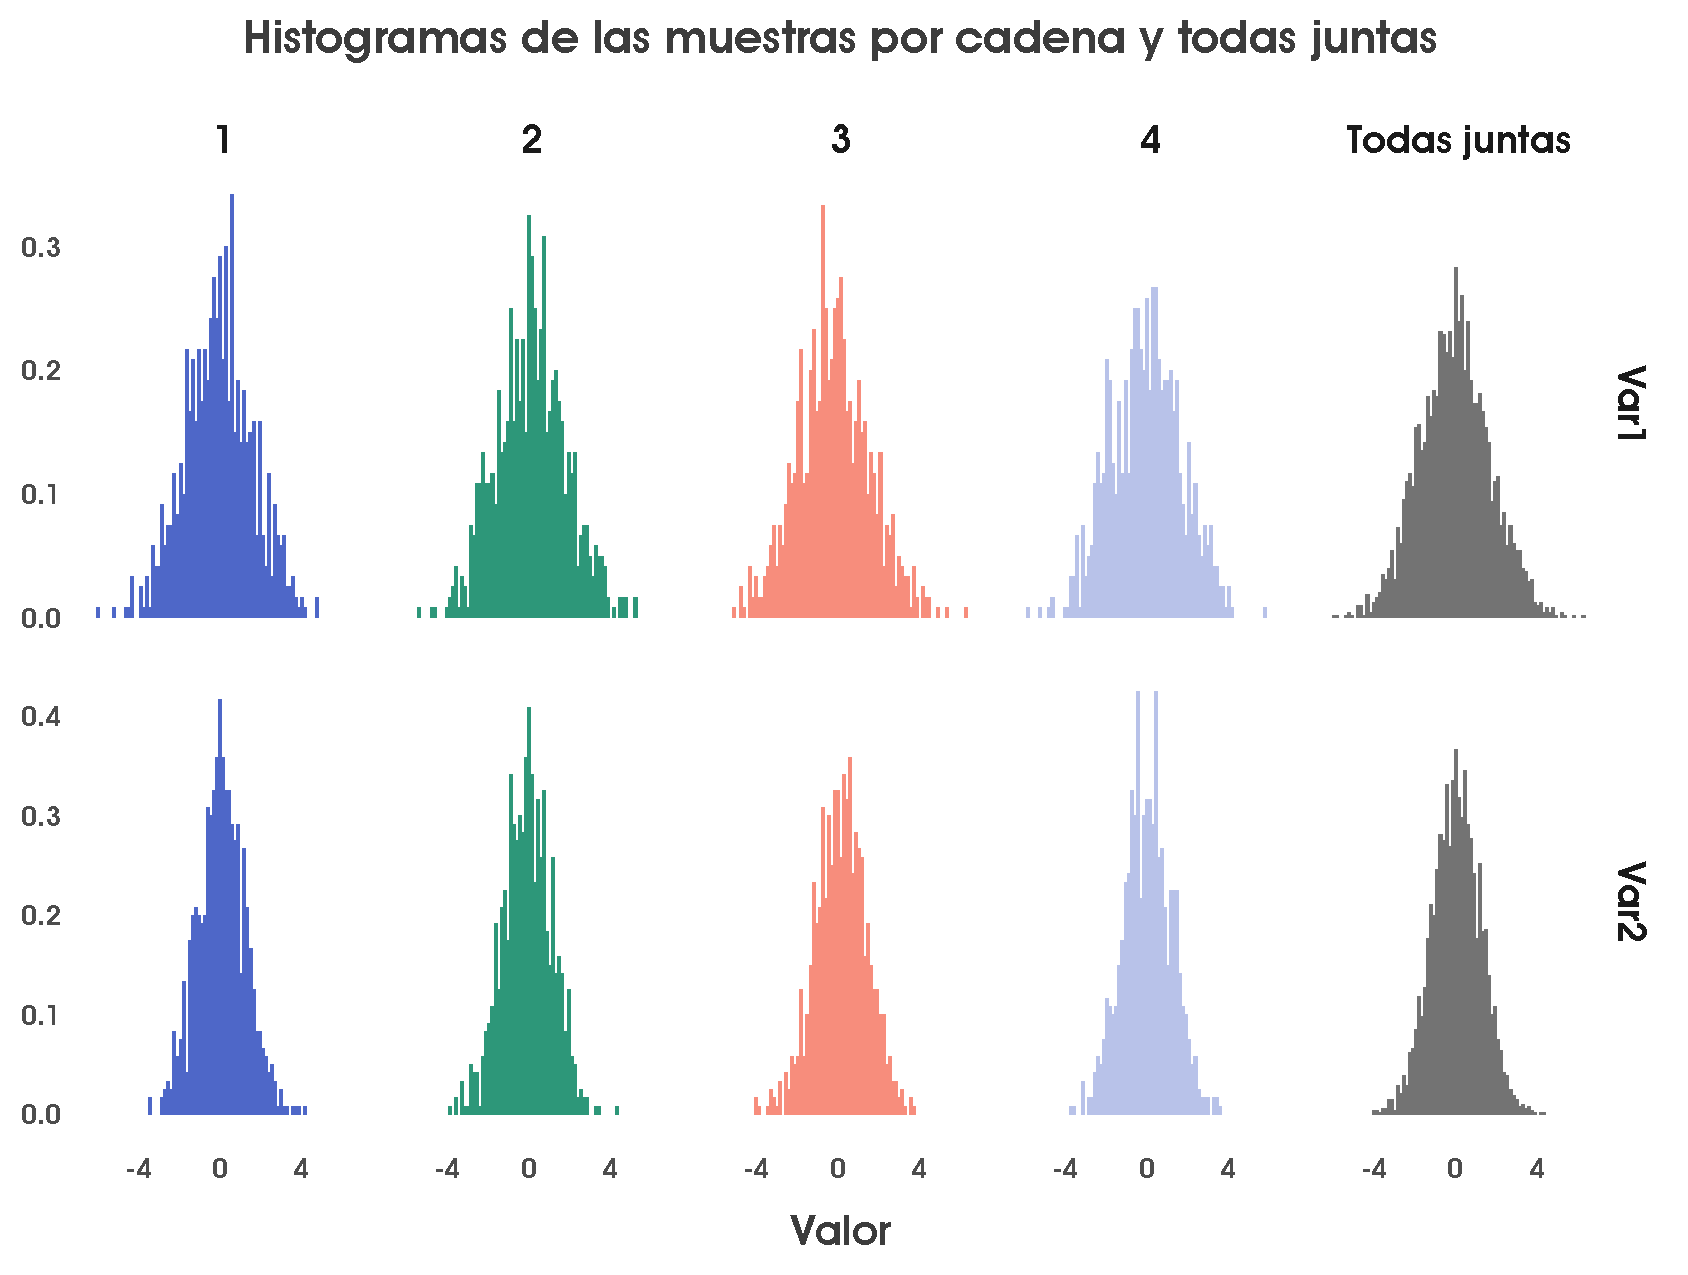
\includegraphics[width=0.9\textwidth]{Figs/Bayes/Ejemplos_Convergencia_Histogramas}
	\caption{Comparación de histogramas para las 4 cadenas de \textit{Gibbs Sampling} considerando solo las iteraciones válidas. Fuente: elaboración propia.}
	\label{fig:Conv_Hist}	
\end{figure}

A pesar de su utilidad, siempre hay que tener presente que los diagnósticos gráficos pueden ser engañosos y no bastan por si solos. Si la distribución es multimodal, por ejemplo, los gráficos de oruga pueden no mezclarse porque cada cadena explora una moda distinta.\\ 

Por otro lado, existen también resúmenes estadísticos para evaluar convergencia. Una estadística frecuentemente utilizada y que es normalmente reportada en softwares de cómputo mediante MCMC es el \textit{factor de reducción de escala} $\hat{R}$ propuesto por \textcite{GelmanRubin92}. Este está basado en comparar las varianzas de los parámetros o resúmenes inferenciales a través de las cadenas con aquellos dentro de cada cadena. La $\hat{R}$, bajo supuestos de normalidad, tiende a 1 conforme la convergencia aumenta. Por ello, un valor empírico cercano a 1, es normalmente requerido antes de poder declarar la convergencia.\\

Finalmente, querría comentar que hay 3 factores principales que permiten tener un buen muestreador de MCMC \parencite{Neal93}. El primero es la cantidad de cómputo requerida para simular cada transición; esta, por ejemplo, podría ser una ventaja de \textit{Gibbs Sampling} sobre \textit{Random Walk Metropolis} pues al aceptar todas las propuestas nos ahorramos la necesidad de realizar la corrección de Metropolis. El segundo factor es el tiempo que le lleva a la cadena alcanzar la convergencia; esto indica de manera general la cantidad de cómputo invertido en el periodo de calentamiento que se descartará. El tercer y útlimo factor está relacionado con el segundo pero es ligeramente diferente: las transiciones necesarias para movernos de un estado en la distribución objetivo a otro prácticamente independiente. Esto nos indicará el tamaño de la simulación requerido para realizar una estimación con alguna precisión deseada. Es normalmente este tercer factor el que motiva el uso de un muestreador distinto a RWM o a \textit{Gibbs Sampler} y que en esta tesis resulta ser \textit{Hamiltonian Monte Carlo}.\label{factor_ventaja_HMC}

